\PassOptionsToPackage{unicode,pdfusetitle}{hyperref}
\PassOptionsToPackage{hyphens}{url}
\PassOptionsToPackage{dvipsnames,svgnames,x11names}{xcolor}

\documentclass[aspectratio=1610]{beamer}

\usetheme{moloch}
\usefonttheme{professionalfonts}
\setbeamertemplate{page number in head/foot}[appendixframenumber]

\usepackage{lmodern}
\usepackage{amssymb,amsmath,mathtools,amsthm}
\usepackage[T1]{fontenc}
\usepackage{textcomp}

\usepackage{upquote} % straight quotes in verbatim environments
\usepackage{microtype}
\UseMicrotypeSet[protrusion]{basicmath} % disable protrusion for tt fonts

\usepackage{xcolor}
\usepackage{xurl} % add URL line breaks if available
\usepackage{bookmark}
\usepackage{hyperref}

\hypersetup{%
  colorlinks = true,
  linkcolor  = mLightGreen,
  filecolor  = mLightGreen,
  citecolor  = mLightGreen,
  urlcolor   = mLightGreen
}

% % animations
% \usepackage{xmpmulti}

%% subfigures
% \usepackage{subcaption}

% algorithms
\usepackage[ruled,vlined]{algorithm2e}
\resetcounteronoverlays{algocf}

\usepackage{booktabs}

\date{\today}
\titlegraphic{\hfill
\includegraphics[width=4cm]{images/ucph-horizontal-right.pdf}\vspace{1cm}}

% % bibliography
% \usepackage[style=authoryear]{biblatex}
% \addbibresource{lecture12.bib}

% title block
\title{Variations on Stochastic Gradient Descent}
\subtitle{Computational Statistics}
\author{Johan Larsson}
\institute{Department of Mathematical Sciences, University of Copenhagen}

% operators
\DeclareMathOperator*{\argmax}{arg\,max}
\DeclareMathOperator{\diag}{diag}

% macros
\newcommand{\pkg}[1]{\textsf{#1}}
\renewcommand{\vec}{\vectorsym}
\newcommand{\mat}{\matrixsym}
\newcommand{\du}{\mathrm{d}}


\begin{document}

\maketitle

% \begin{frame}[c]
%   \frametitle{Overview}
%
%   \tableofcontents
% \end{frame}

\begin{frame}[c]
  \frametitle{Stochastic Gradient Descent}

  \begin{columns}
    \begin{column}{0.45\textwidth}
      \begin{block}{Last Time}
        Introduced stochastic gradient descent (SGD) and mini-batch version thereof.
      \end{block}
      \only<2->{
        \begin{block}{Problems}
          We indicated that there were problems with vanilla SGD: poor convergence,
          erratic behavior.
        \end{block}
      }
    \end{column}
    \begin{column}{0.45\textwidth}
      \begin{algorithm}[H]
        \SetAlgoLined
        \KwData{$\gamma_0 >0$ }
        \Repeat{convergence}{
          $A_k \gets$ random mini-batch of $m$ samples\;
          $x_k \gets x_{k-1} - \frac{\gamma_k }{|A_k|} \sum_{i \in A_k} \nabla f_i(x_{k-1})$\;
        }
        \caption{Mini-Batch SGD}
      \end{algorithm}
    \end{column}
  \end{columns}

\end{frame}

\begin{frame}[c]
  \frametitle{Today}

  How can we improve stochastic gradient descent?

  \begin{block}{Momentum}
    Base update on combination of gradient step and previous point.
  \end{block}

  \pause

  \begin{block}{Adaptive Gradients}
    Adapt learning rate to particular feature.
  \end{block}

\end{frame}

\begin{frame}[c]
  \frametitle{Momentum}

  \begin{figure}[htpb]
    \centering
    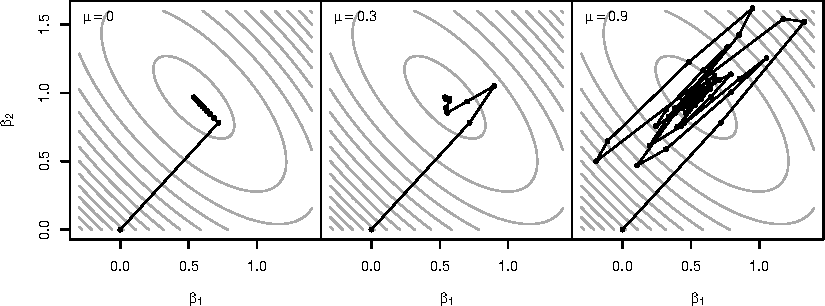
\includegraphics[]{images/momentum-surface.pdf}
    \caption{%
      Trajectories of GD for different momentum values
    }
    \label{fig:momentum-surface}
  \end{figure}

\end{frame}

% \begin{frame}[standout]
%   Thank you!
% \end{frame}

% \appendix
% 
% \begin{frame}[allowframebreaks]{References}
%   \printbibliography[heading=none]
% \end{frame}

\end{document}

